\documentclass[preprint,3p]{elsarticle}
%\documentclass[preprint]{aastex}
\usepackage{aas_macros}
\usepackage{amsmath,amssymb}
\usepackage{mathrsfs}
\usepackage{graphicx}
\usepackage{bm}
\usepackage{hyperref}
\DeclareMathOperator\erf{erf}
\newcommand{\mli}[1]{\mathit{#1}}
%\usepackage{epstopdf}


\begin{document}

%\begin{frontmatter}
%
%\title{Toy Model}
%\author{A.~G. Kim\corref{cor1}}
%\ead{agkim@lbl.gov}
%\address{Physics Division, Lawrence Berkeley National Laboratory, 1 Cyclotron Road, Berkeley CA, USA 94720}
%
%\begin{abstract}
%\end{abstract}
%\begin{keyword}
%\end{keyword}
%\end{frontmatter}

\section{Likelihood}
\label{likelihood:sec}

The ambition is to construct a model to determine the likelihood of DES-like
supernova data.  We start with a toy model and plan to evolve its complexity to
have the fidelity necessary for the DES analysis.
The conceptual structure of the model is shown in Figure~\ref{pgm:fig}. 
\begin{figure}[htbp] %  figure placement: here, top, bottom, or page
   \centering
   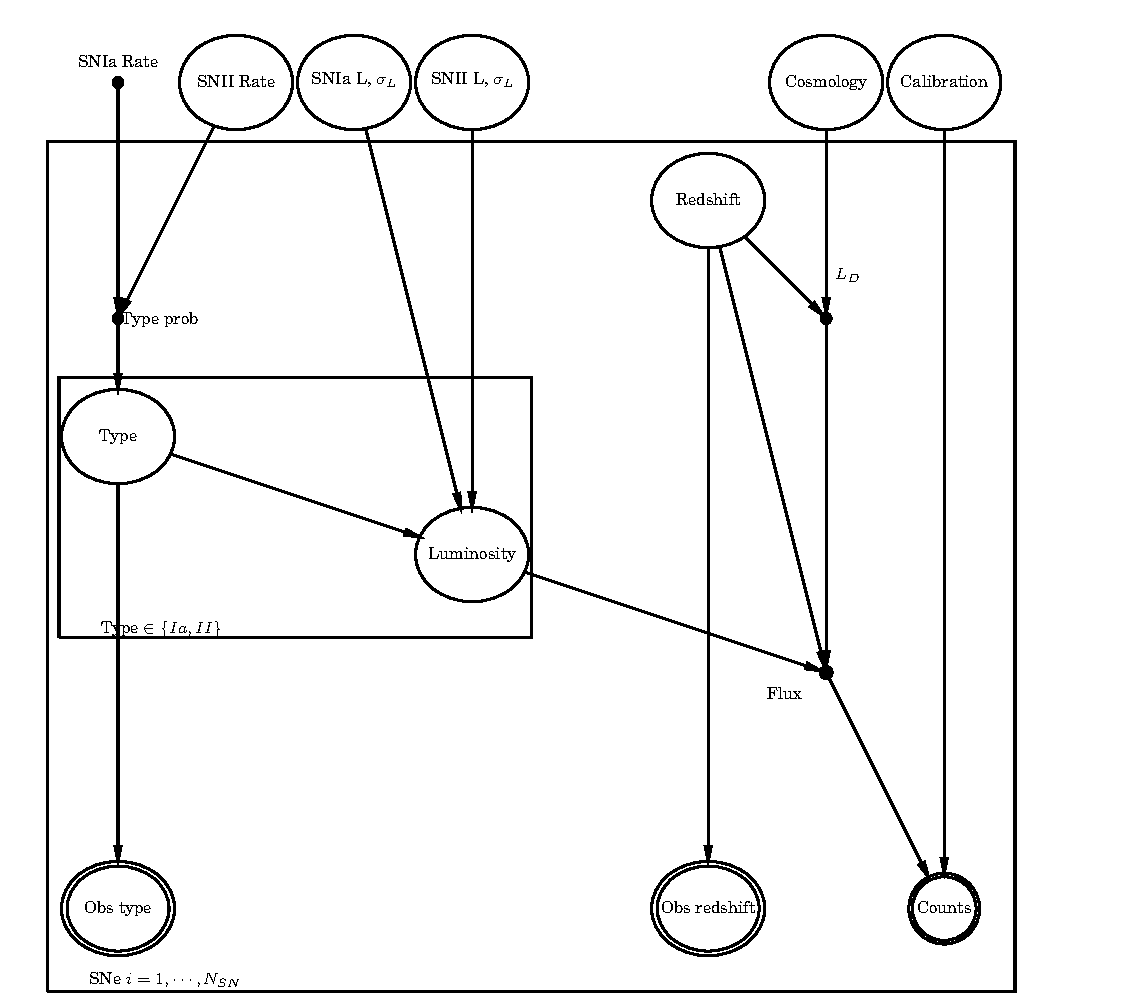
\includegraphics[width=6.5in]{../results//nodes_pgm.pdf} 
   \caption{Probabilistic Graphical Model for the SN~Ia analysis.  
   \label{pgm:fig}}
\end{figure}

In the toy model there are three types of data that
may be observed for each supernova:
\begin{itemize}
\item $c_o$: Counts at peak brightness, one or more independent measurements.
\item $z_o$: Redshift.
\item $T_o$: Transient type.
\end{itemize}

There are selection criteria $S_c$ and $S_T$ for the inclusion of an object in the
sample and for a successul typing.
In what follows we assume that the typed objects are drawn from the same underlying
distribution as the sample $S_c=S_T$, and that the selection criterion depends on a  brightness
threshold $S_c = c_o \ge c_T$.  (The spectroscopic sample $S_T$ 
eventually should depend on the
photometry and the quality of the spectroscopic data.)

For this preliminary discussion the top-level parameters are denoted by $X$,
the latent parameters are $L$ and $T$ (for luminosity and type).  

It is useful to split the data into two cases depending on whether or not
the transient has a type measurement $T_o$.

\subsection{Case Typed}
For Case Typed the likelihood is
\begin{align}
\mathcal{L}(T_o,z_o,c_o | S_c, S_T, z, X) & =  \int dL \sum_i p(T_o,z_o,c_o | T_i, L, S_c, S_T, z, X) p(L |  T_i,  S_c, S_T, z, X) P(T_i|S_c, S_T, z, X).
\end{align}
We assume that the observations give a perfect measurement of type and redshift,
so that
\begin{align}
p(T_o|T) & =\delta(T_o-T)\\
p(z_o|z) & =\delta(z_o-z);
\end{align}
$T$ and $z$ are no longer probabilistic but are fixed.
Then
\begin{align}
\mathcal{L}(T_o,z_o,c_o | S_c, S_T, z, X) & =  \int dL\, p(c_o | T=T_o, L, S_c, S_T, z=z_o, X) p(L| T=T_o, S_c, S_T, z=z_o, X)  P(T_o|S_c, S_T, z=z_o, X) \\
&= \int dL\, \frac{ p(c_o, S_c, S_T | T=T_o, L, z=z_o, X) }{P(S_c, S_T, | T=T_o, L,  z=z_o, X) }
\frac{p(L, S_c, S_T | T=T_o, z=z_o, X)}{P(S_c, S_T| T=T_o,  z=z_o, X)}
\frac{p(T_o, S_c, S_T | z=z_o, X)}{P(S_c, S_T| z=z_o, X)} \\
&= \frac{\int dL\, p(L|T_o, z=z_o, X) P(T_o|z=z_o, X) p(c_o, S_c, S_T | T=T_o, L, z=z_o, X)}{P(S_c, S_T| z=z_o, X)}.%\\
%&= \frac{\int dL\, p(L|T_o, z=z_o, X) P(T_o|z=z_o, X) p(c_o | T=T_o, L, z=z_o, X)}{P(S_c, S_T| z=z_o, X)}.
\end{align}

The photometric and spectroscopic sample selections can be treated as efficiencies $\epsilon_c$, $\epsilon_T$ as
\begin{align}
p(c_o, S_c, S_T | T=T_o, L, z=z_o, X) & = \int ds\, p(c_o, s, S_c, S_T | T=T_o, L, z=z_o, X) \\
 & =p(c_o, S_c | T=T_o, L, z=z_o, X)  \int ds\,  p(s, S_T | T=T_o, L, z=z_o, X) \\
 & = \epsilon_c(c_o) p(c_o| T=T_o, L, z=z_o, X)  \int ds\, \epsilon_T(c_o, s)  p(s | T=T_o, L, z=z_o, X) \\
 & \approx \epsilon_c(c_o)   \epsilon_T(c_o, s_\star) p(c_o| T=T_o, L, z=z_o, X).
\end{align}
where the supernova signal in the spectrum $s$ is not extracted and we make the approximation $ p(s | T=T_o, L, z=z_o, X)  = \delta(s-s_\star)$
and $s_\star(t_T; T=T_o, L, z=z_o, X)$ is the expected signal.


The  normalization term sums/integrates over all possible observed types/counts 
\begin{align}
P(S_c, S_T| z=z_o, X) & =\sum_i \int dc_o \mathcal{L}(T_i,z_o,c_o | S_c, S_T, z, X) \\
% & =\sum_i \int_{-\infty}^{\infty} dc_o \mathcal{L}(T_i,z_o,c_o | S_c, S_T, z, X) \\
%& = \sum_i \int_{c_T}^{\infty} dc_o \mathcal{L}(T_i,z_o,c_o | S_c, S_T, z, X)\\
& = \sum_i  P(T_i|z=z_o, X)\int dL\, p(L|T_i, z=z_o, X)  \left[\int dc_o\,  p(c_o,S_c, S_T | T=T_i, L, z=z_o, X)\right] \\
& \approx  \sum_i   P(T_i|z=z_o, X)\int dL\, p(L|T_i, z=z_o, X)  \left[ \int dc_o\, \epsilon_c(c_o)  \epsilon_T(c_o, s_\star)  p(c_o| T=T_o, L, z=z_o, X)  \right] .
\end{align}

\subsection{Case Not Typed}


For Case Not Typed the likelihood is
\begin{align}
\mathcal{L}(z_o,c_o | S_c, S_T, z, X) & =  \int dL \sum_i p(z_o,c_o | T_i, L, S_c, S_T, z, X) p(L |  T_i,  S_c, S_T, z, X) P(T_i|S_c, S_T, z, X).
\end{align}

For the redshift measurement, we take a set of potential host galaxies, where galaxy $j$
are redshift $z_j$ has probability $p_j$ of being the host
\begin{equation}
p(z_o|S_c, S_T, z, X) = \sum_j   p_j\delta(z_j-z).
\end{equation}
Then
\begin{align}
\mathcal{L}(z_o,c_o | S_c, S_T, z, X) & =  \sum_j p_j \int dL \,\sum_{i} p(c_o | T_i, L, S_c, S_T, z=z_j, X) p(L |  T_i,  S_c, S_T,  z=z_j, X) P(T_i|S_c, S_T, z=z_j, X) \\
&=  \frac{\sum_j p_j \int dL \, p(c_o, S_c, S_T | L, z=z_j, X) \sum_{i}  p(L|T_i, z=z_j, X) P(T_i|z=z_j, X)   }{P(S_c, S_T| z=z_j, X)}\\
&=  \frac{\sum_j p_j \int dL \, p(c_o | L, z=z_j, X) \sum_{i}  p(L|T_i, z=z_j, X) P(T_i|z=z_j, X)   }{P(S_c, S_T| z=z_j, X)},
\end{align}
where we use the fact that the counts do not directly depend on type.

The normalization term is
\begin{align}
P(S_c| z=z_o, X) & = \int dc_o \, \mathcal{L}(T_i,z_o,c_o | S_c, S_T, z, X)\\
& =  \sum_j p_j  \sum_{i} P(T_i|z=z_j, X)  \int dL \, p(L|T_i, z=z_j, X) 
\left[ \int dc_o \, p(c_o, S_c| T=T_i, L, z=z_j, X) \right].
\end{align}

\subsection{Sample Selection}
Both the Typed and Not Typed cases have in their normalizations the term
\begin{equation}
\int dc_o \, p(c_o,S_c, S_T | T=T_i, L, z=z_o, X),
\end{equation}
which is the fraction of objects whose counts satisfy the sample selection criteria.


In the case of a single count measurement per transient and neglecting the typing selection criteria,
\begin{align}
 p(c_o, S_c, S_T | T=T_o, L, z=z_o, X) &=  p(c_o, c_o \ge  c_T | T=T_o, L, z=z_o, X) \\
 &= \begin{cases}
   p(c_o | T=T_o, L, z=z_o, X) & \text{if } c_o \ge c_T \\
   0 & \text{if }  c_o < c_T
 \end{cases}
\end{align}
so that the integral is
\begin{equation}
\int dc_o \, p(c_o,S_c, S_T | T=T_i, L, z=z_o, X) = \int_{c_T}^\infty dc_o\,  p(c_o | T=T_i, L, z=z_o, X).
\end{equation}
Our count measurements come from a Normal distribution, so that integral is simply related to the error function.

For the more general case, suppose a transient has $N$ independent count measurements\footnote{The independence of count measurements  depends on the flux extraction method; regardless the
noise of a single observation is expected to be dominated by its own photon noise making this
supposition a good approximation.} and $k$ of those must be above threshold in order to be
included in the sample.
Consider arrays of length $N$ in which each element has a value of True or False: there are $2^N$ possible configurations for this array
of which $\sum_{i=k}^N {N \choose i}$ have $k$ or more True's.  Let the set $\mathcal{G}$ represent the latter possible configurations.
Then
\begin{align}
p(c_o, S_c| T=T_o, L, z=z_o, X) &= \sum_{g \in \mathcal{G}} \prod_{\alpha} p(c_{o, \alpha}, g | T=T_o, L, z=z_o, X)\\
 &=  \sum_{g \in \mathcal{G}}  \prod_{\alpha} \begin{cases}
   p(c_{o,\alpha} | T=T_o, L, z=z_o, X) & \text{if } (c_{o,\alpha} \ge c_T) = g_\alpha\\
   0 & \text{if }  (c_{o,\alpha} \ge c_T)  \ne g_\alpha
 \end{cases}
\end{align}
and the normalization integral is composed of the sum over all possible configurations of the integrated probability of the truncated distributions
of the measured counts.  This simplifies to the the single-count case considered earlier in the case of $N=1$, $k=1$.
If the count measurement uncertainties are independent, which may not be exactly but is approximately the case when we have high
signal-to-noise references, the integral because a sum of products of normalized error functions.



\section{Model}
\label{model:sec}

We now go into more detail into the model and the form of the pdf's that enter
into the likelihoods described in \S\ref{likelihood:sec}.

A description of the nodes follow.  Numbers are illustrative. 

\subsection{Cosmology}
The Flat $w$CDM cosmological parameters are drawn from top-hat distributions
\begin{align}
\Omega_M & \sim  {\mathcal{U}}(0,1)\\
w_0 & \sim \mathcal{U}(-1.5, -0.1).
\end{align}


\subsection{Calibration}
Photometric zeropoints for each band.
\begin{equation}
Z \sim \mathcal{N}(0,\frac{\ln{10}}{2.5}0.01)
\end{equation}

\subsection{SNIa Rate}
Type~Ia SN rate. In the analysis only relative rates between different transients are important.
We take the rates relative to the SN~Ia rate
\begin{equation}
r_{SNIa} = 1.
\end{equation}

\subsection{SNII Rate}
Type~II SN rate, relative to the SN~Ia rate
\begin{equation}
r_{SNII} \sim \mathcal{U}(0.25, 4).
\end{equation}

\subsection{SNIa Luminosity}
The mean luminosity and intrinsic dispersion for SNe~Ia. In fact work with log-luminosity, intrinsic
dispersion in mag units.
\begin{align}
\ln{L}_{SNIa} & \sim \mathcal{N}(\ln{1}, 0.02) \\
\sigma_{SNIa} & \sim \ln{\mathcal{N}}(\ln{0.1},0.1).
\end{align}

\subsection{SNII Luminosity}
The mean luminosity and intrinsic dispersion for SNe~II. In fact work with log-luminosity, intrinsic
dispersion in mag units.
\begin{align}
\ln{L}_{SNII} & \sim \mathcal{N}(\ln{0.5}, 0.02) \\
\sigma_{SNII} & \sim \ln{\mathcal{N}}(\ln{0.4},0.1).
\end{align}

\subsection{SNIa~Probability}
Probability an object is SN~Ia
\begin{align}
p_{SNIa} &= \frac{r_{SNIa}}{r_{SNIa}+r_{SNII}} \nonumber \\
p_{SNII}&=1-p_{SNIa}.
\label{prob:eqn}
\end{align}
\subsection{Type}
The type of the object $T$ is drawn from the Bernoulli distribution 
\begin{equation}
T | p_{SNIa} \sim \mathcal{B}(1-p_{SNIa}),
\end{equation}
with the convention that $T=0$ corresponds to SN~Ia.

The type probability appears explicitly in the calculation of the likelihoods.
\begin{align}
P(T_{SNIa} | z=z_j, X) &= p_{SNIa}\\
P(T_{SNII} | z=z_j, X) &= p_{SNII}
\end{align}
\subsection{Observed Type}
The observed type is assumed to be perfect.
\begin{equation}
T_o = T.
\end{equation}

\subsection{Luminosity}
For our model
\begin{equation}
\ln{L} | T, \ln{L}_{T},\sigma_{T} \sim \mathcal{N}\left( \ln{L}_{T},\frac{\ln{10}}{2.5}\sigma_{T}\right).
\end{equation}

The corresponding pdf appears in the likelihood.

\subsection{Redshift}
The redshift is drawn from a flat distribution
\begin{equation}
z\sim \mathcal{U}(0,\infty).
\end{equation}
%
%\subsection{Neighbor Galaxy Redshifts}
%Each neighbor redshift is drawn from a flat distribution.  The redshift for neighbor
%$i$ is  
%\begin{equation}
%z_{N,i} \sim \mathcal{U}(0,\infty).
%\end{equation}

\subsection{Observed Redshift}
In our model the measured redshift is a sum of delta functions
\begin{equation}
p(z_o|z) = \sum_i p_i \delta(z-z_i),
\end{equation}
where galaxy $i$ at
redshift $z_i$ has probability $p_i$ of being
the host.  

\subsection{Counts}
The luminosity distance comes from the physics-theory function
\begin{equation}
d_L = d_L(z; \Omega_M, w0),
\end{equation}
the flux is
\begin{equation}
f = \frac{L}{4\pi d_L^2},
\end{equation}
and expected counts is
\begin{equation}
c_\star = 10^{Z/2.5}f.
\end{equation}
The distribution of counts for all transients is 
\begin{equation}
c_o | c_\star, \sigma_c \sim \mathcal{N}(c_\star, \sigma_c),
\end{equation}
where $\sigma_c$ is the measurement noise.

\subsection{Implementation Notes}
Anticipating the use of available statistical packages, the likelihoods have been constructed
from standard distribution functions.  The truncated distributions from sample selection
are accounted by the normalization 
terms $P(S_c, S_T| z=z_o, X)$, $P(S_c| z=z_o, X)$.  Although they do not appear
in the PGM, they are treated as nodes who contribute 
$-\ln{P(S_c, S_T| z=z_o, X)}$ to the log-likelihood, where the negative sign reflects that this is a normalization
factor.


The following integral appears in the normalization
\begin{equation}
\int dL p(L|T_i, z=z_o, X)  \left[\int_{c_T}^{\infty} dc_o  p(c_o | T=T_i, L, z=z_o, X)\right].
\end{equation}
We actually work with $\ln{L_X}$ and $\sigma_X$.  Setting
\begin{equation}
n=\frac{\ln{L}-\ln{L_X}}{\sigma_X}
\end{equation}
the integral becomes
 \begin{equation}
\sigma_X \int dn p(n\sigma_X + \ln{L_X} |T_i, z=z_o, X)  \left[\int_{c_T}^{\infty} dc_o  p(c_o | T=T_i, L_Xe^{n\sigma_X}, z=z_o, X)\right].
\end{equation}
The two probability distributions are normal so that this reduces to
 \begin{equation}
\frac{1}{2\sqrt{2\pi}} \int dn\, e^{-0.5n^2} \left(1-erf\left(\frac{(c_T - c_\star)}{\sqrt{2}\sigma_c}\right)\right),
\end{equation}
where
\begin{equation}
c_\star = \frac{e^{\ln{L_X}+n\sigma_X}}{4\pi d_L^2}10^{Z/2.5}.
\end{equation}

\section{Adding Complexity}
\subsection{SALT2 Model for Transient Luminosity}
The SALT2 model for supernova luminosity as a function of SN-frame time $t$  and wavelength $\lambda$ is
\begin{equation}
L(t-t_0, \lambda; M-x_0-\alpha x_1 + \beta c, x_1, c),
\label{SALTL:eqn}
\end{equation}
where $\alpha$ and $\beta$ are global parameters and $t_0$, $x_0$, $x_1$ and $c$ are per-supernova parameters.

Incorporating the SALT2 model leads to changes to the PGM in Figure~\ref{pgm:fig}, specifically in the following Nodes.
UNITY notation and priors are taken.
\subsubsection{SNX Luminosity}
There are parameters for the global supernova parameters.  For SNe~Ia
\begin{align}
M_{SNIa} & \sim \mathcal{U}(-20, -18) \\
\arctan{\alpha_{SNIa}} & \sim \mathcal{U}(-0.2, 0.3) \\
\arctan{\beta_{SNIa}} & \sim \mathcal{U}(-1.4, 1.4)
\end{align}
and for ``hyperparameters'' that describe the distributions of the per-supernova parameters
\begin{align}
\log_{10}{R^{x_0}_{SNIa}} & \sim \mathcal{U}({-2}, {-0.5})\\
\log_{10}{R^{x_1}_{SNIa}} & \sim \mathcal{U}({-0.5}, {0.5})\\
\log_{10}{R^{c}_{SNIa}} & \sim \mathcal{U}({-1.5}, {-0.5})\\
x_{1,SNIa}^\star& \sim \text{Cauchy}(0,1)\\
c^\star_{SNIa} & \sim \text{Cauchy}(0,0.3).
\end{align}


\subsubsection{Type}
The type of the object is still obtained as before.  Now we have the parameters that specify the sub-type.
\begin{align}
t_0 & \sim \mathcal{U}\\
x_{0, SNIa} & \sim \mathcal{N}(0,R^{x_0}_{SNX})\\
x_{1,SNIa} & \sim \mathcal{N}(x_{1,SNIa}^\star,R^{x_1}_{SNIa})\\
c_{SNIa} & \sim \text{SkewNormal}(c^\star_{SNIa},R^{c}_{SNIa} )
\end{align}

\subsubsection{Luminosity}
The luminosity is now fixed by Eqn.\ \ref{SALTL:eqn}.  It may be made probabilistic if an error snake is considered.

\subsubsection{Likelihood}
The likelihood for typed objects is
\begin{multline}
\mathcal{L}(T_o,z_o,c_o | S_c, S_T, z, X)
 \propto \int dt_0 \, dx_{0,T_o} \, dx_{1,T_o} dc_{T_o} 
 p(t_0, x_{0,T_o}, x_{1,T_o}, c_{T_o} |T_o, z=z_o, X) \\ P(T_o|z=z_o, X) p(c_o, S_c, S_T | T=T_o, L_{T_o}(t_0, x_{0,T_o}, x_{1,T_o}, c_{T_o}), z=z_o, X)
\end{multline}
and for non-typed
\begin{multline}
\mathcal{L}(z_o,c_o | S_c, S_T, z, X)
 \propto \sum_j p_j \sum_i P(T_i|z=z_j, X)   \int dt_0 \, dx_{0,T_i} \, dx_{1,T_i} dc_{T_i} 
 p(t_0, x_{0,T_i}, x_{1,T_i}, c_{T_i} |T_i, z=z_j, X) \\  p(c_o, S_c, S_T | T=T_o, L_{T_i}(t_0, x_{0,T_i}, x_{1,T_i}, c_{T_i}), z=z_j, X),
 \end{multline}
where both likelihoods must be normalized.

\end{document}